%!TEX root = ../template.tex
%%%%%%%%%%%%%%%%%%%%%%%%%%%%%%%%%%%%%%%%%%%%%%%%%%%%%%%%%%%%%%%%%%%
%% chapter1.tex
%% NOVA thesis document file
%%
%% Chapter with introduction
%%%%%%%%%%%%%%%%%%%%%%%%%%%%%%%%%%%%%%%%%%%%%%%%%%%%%%%%%%%%%%%%%%%

\typeout{NT FILE chapter2.tex}%

\chapter{Background}
\label{chap:back}
In this chapter, we will provide the necessary context to understand the main concepts explored throughout this document. We begin with an introduction to logic focusing on Propositional Logic and First-Order Logic. For each of these logic branches, we will describe briefly its syntax and semantics. With this basic knowledge as a foundation, we will then introduce Natural Deduction, a fundamental topic for this work, as it explains what it is and presents examples of the types of exercises we will develop. Finally, we will discuss proof assistants, with a particular focus on Isabelle/HOL and Lean, exploring how these tools can help us in developing our feedback system.

\section{Propositional Logic}
\label{chap:prop}
Logic in general is defined as the study of the principles of reasoning. \gls{PL} is a branch of logic that focuses on the study of propositions and their relationships. The goal of logic in computer science is to create languages that help us represent situations we deal with as computer scientists. These languages allow us to think about and analyze situations in a structured way. By using logic, we can build clear and valid arguments about them, ensuring they make sense and can be tested, defended, or even carried out by a machine~\cite{huth_2004_logic}. Propositions are the basic building blocks of \gls{PL}. A proposition is a declarative statement that has a truth value, which can be either true (denoted as T or 1) or false (denoted as F or 0), but not both.

\textbf{Examples of Propositions:}
\begin{center}
    \textbf{p:} "It is raining." \quad \textbf{q:} "It is cold." \quad \textbf{r:} "It is snowing."
\end{center}

To define a formal language, one must choose the alphabet of the language and establish the set of words that make up the language. These words are usually called formulas when the formal language is associated with a logic, as is the case here. The alphabet of the language is a set of symbols that, when combined, form formulas, with each formula being a finite sequence of symbols from the alphabet~\cite{gouveia_lgica}. In \gls{PL}, we have propositional symbols, conventionally represented by lowercase letters (\(p\), \(q\), \(r\)), and symbols that represent relations between propositions (\(\neg\), \(\land\), \(\lor\), \(\to\), \(\leftrightarrow\)), also known as logical connectives. To represent generic formulas, we use Greek letters (\(\phi\), \(\psi\), \(\gamma\)). Another important symbol in \gls{PL} is parentheses, which help resolve ambiguities in formulas, similar to their use in mathematics to indicate operation priority. Additionally, we have two constants, one to represent truth, (\(\top\)), and one to represent falsehood (\(\bot\)).

For the sake of interpretation, we will use the propositions (\(p\), \(q\) and \(r\)) introduced in the previous example in the following explanations. \autoref{tab:logical_constants_and_prop_vars} and \autoref{tab:logical_connectives} list all the logical constants and connectives of the \gls{PL} alphabet.

\begin{table}[h!]
    \centering
    \resizebox{\textwidth}{!}{ 
    \begin{tabular}{|c|p{6cm}|p{8cm}|}
    \hline
    \textbf{Symbol} & \textbf{Name} & \textbf{Value} \\ \hline
    \(\top\) & Top  & True or 1\\ \hline
    \(\bot\) & Bottom & False or 0\\ \hline
    \end{tabular}}
    \caption{Logical constants in Propositional Logic}
    \label{tab:logical_constants_and_prop_vars}
\end{table}

\begin{table}[h!]
    \centering
    \resizebox{\textwidth}{!}{
    \begin{tabular}{|c|p{6cm}|c|p{8cm}|}
    \hline
    \textbf{Symbol} & \textbf{Name} & \textbf{Arity} & \textbf{Example} \\ \hline
    \(\neg\) & Not & 1 & \(\neg p\): "It is not raining." \\ \hline
    \(\land\) & And & 2 & \(p \land q\): "It is raining and it is cold." \\ \hline
    \(\lor\) & Or & 2 & \(p \lor q\): "It is raining or it is cold." \\ \hline
    \(\to\) & Implication & 2 & \(p \to q\): "If it is raining, then it is cold." \\ \hline
    \(\leftrightarrow\) & Equivalence & 2 & \(p \leftrightarrow q\): "It is raining if and only if it is cold." \\ \hline
    \end{tabular}}
    \caption{Logical connectives in Propositional Logic}
    \label{tab:logical_connectives}
\end{table}

We have defined the symbols that make up the \gls{PL} alphabet. Now, we will specify which sequences of these words are valid by defining \gls{WFF}. A \gls{WFF} in \gls{PL} is defined inductively using a set of rules that specify the conditions for a formula to be considered well-formed. These rules build upon each other, allowing for the construction of more complex logical expressions.

\[
\left\{
\begin{array}{ll}
\top \text{ is a WFF,}\\
\bot \text{ is a WFF,}\\
\alpha \text{ is WFF} & \text{if } \alpha \text{ is a proposition,}\\
\neg \alpha \text{ is a WFF} & \text{if } \alpha \text{ is a WFF,}\\
(\alpha \land \beta) \text{ is a WFF} & \text{if } \alpha \text{ and } \beta \text{ are WFFs,}\\
(\alpha \lor \beta) \text{ is a WFF} & \text{if } \alpha \text{ and } \beta \text{ are WFFs,} \\
(\alpha \rightarrow \beta) \text{ is a WFF} & \text{if } \alpha \text{ and } \beta \text{ are WFFs,} \\
(\alpha \leftrightarrow \beta) \text{ is a WFF} & \text{if } \alpha \text{ and } \beta \text{ are WFFs} \\
\end{array}
\right.
\]

\textbf{Examples of WFF:}
\begin{itemize}[itemsep=2pt]
    \renewcommand{\labelitemi}{}
    \item \(\top\): "True".
    \item \(((p \land q) \to r)\): "If it is raining and it is cold, then it is snowing."
    \item \(((p \to q) \land (q \to r))\): "If it is raining, then it is cold, and if it is cold, then it is snowing."
\end{itemize}

To define a language, we also need to define its semantics. In \gls{PL}, this is no different. Given a formula, we want to determine its truth value, which depends on the truth values of its propositional symbols. To do so, we must define an interpretation or valuation (\(V\)), which is a function that associates a truth value with each propositional symbol in a set (\(P\)), formally \(V: P \to \{0,1\}\)~\cite{gouveia_lgica}. We say that a formula \(\varphi\) is satisfiable by an interpretation if the interpretation satisfies the formula (if it evaluates to true in that interpretation), denoted by \(V \Vdash \varphi\). Otherwise, the formula is not satisfiable under that interpretation, denoted by \(V \nVDash \varphi\). 

\[
\left\{
\begin{array}{ll}
    V \Vdash \top \text{,}\\
    V \Vdash p  & \text{if } p \text{ is a proposition and its interpretation is true}, \\
    V \Vdash \neg \alpha & \text{if } V \nVdash \alpha \text{,} \\
    V \Vdash (\alpha \lor \beta) & \text{if either } V \Vdash \alpha \text{ or } V \Vdash \beta \text{,} \\
    V \Vdash (\alpha \land \beta) & \text{if both } V \Vdash \alpha \text{ and } V \Vdash  \beta \text{,} \\
    V \Vdash (\alpha \rightarrow \beta) & \text{if whenever } V \Vdash \alpha \text{, then } V \Vdash \beta\text{,} \\
    V \Vdash (\alpha \leftrightarrow \beta) & \text{if both } V \Vdash \alpha \text{ and } V \Vdash \beta \text{ are either both true or both false.}
\end{array}
\right.
\]

With this definition, we can evaluate the nature of a formula.

\begin{itemize}[itemsep=2pt]
    \renewcommand{\labelitemi}{}
    \item \textbf{Possible}: Exists an interpretation that satisfies it.
    \item \textbf{Valid (Tautological)}: Is satisfied by all interpretations.
    \item \textbf{Contradictory}: Is not satisfied by any interpretation.
\end{itemize}

A key task in \gls{PL} and in Logic in general is to determine whether a formula \(\phi\) is a semantic consequence of a set of formulas \(\Gamma\), denoted by \(\Gamma \vdash \phi\)~\cite{gouveia_lgica}. Given a set of premises and a conclusion, the conclusion is considered a semantic consequence of the premises if, for every interpretation of the propositions, whenever the interpretation satisfies all the premises, it must also satisfy the conclusion. In other words, if the set of premises is true under an interpretation, the conclusion must also be true under that interpretation.

\section{First-Order Logic}
\label{chap:fol}
Another branch of logic is \gls{FOL}, also known as predicate logic. Unlike \gls{PL}, which focuses solely on simple declarative statements, \gls{FOL} extends this by introducing new components that enable us to express more complex declarative sentences, capturing relationships between objects and their properties within a specified domain~\cite{huth_2004_logic}. In this context, objects refer to specific entities within the domain of discourse, such as animals, persons, numbers, or things, which can be described or related through properties and predicates.

\textbf{Examples of First-Order Sentences:}
\begin{itemize}[itemsep=2pt]
    \renewcommand{\labelitemi}{}  
    \item "There's a black cat that likes baths." 
    \item "John is a friend of Mary." 
    \item "If a variable is an integer and positive, then it is greater than zero." 
\end{itemize}  

\gls{FOL} extends \gls{PL} syntax by adding features that make it more expressive. It introduces quantifiers, which allow us to generalize or specify expressions, making it possible to express universal truths (\(\forall\)) or existential statements (\(\exists\))~\cite{huth_2004_logic}. Moreover, FOL enables the use of variables, typically represented by (\(x\), \(y\), \(z\)) within a given domain. Predicates, which express properties or relationships, allow \gls{FOL} to capture facts about objects and their interactions. Predicates are represented by words starting with capital letters, such as \( \text{Cat}(x) \), which expresses that \( x \) is a cat. Predicates always return a truth value and can have different arities. We can also define binary relations, such as equality, which is represented by the symbol \( = \). Equality is a binary relation that indicates when two terms refer to the same object in the domain. Similar to predicates, \gls{FOL} includes functions that allow referring to objects in the domain based on other objects in the domain. Functions are represented by words starting with lowercase letters, such as \( \text{father}(x) \), which return a specific value from the domain (e.g., the father of \( x \)). \autoref{tab:pred_var_const_fun} and \autoref{tab:quant} present examples of symbols in \gls{FOL}.


\begin{table}[h!]
    \centering
    \resizebox{\textwidth}{!}{
    \begin{tabular}{|c|p{4cm}|p{10cm}|} 
    \hline
    \textbf{Symbol} & \textbf{Name} & \textbf{Example} \\ \hline
    \(x, y, z\) & Variables & \(x\): "An individual object" \\ \hline
    \(black\) & Constants & \(black\): "Value that is fixed" \\ \hline
    \(Cat(x)\) & Predicates & \(Cat(x)\): "True if \(x\) is a cat" \\ \hline
    \(color(x)\) & Functions & \(color(x) = \text{black}\): "The color of \(x\) is black" \\ \hline
    \end{tabular}}
    \caption{Variables, constants, predicates, and functions in First-Order Logic}
    \label{tab:pred_var_const_fun}
\end{table}

\begin{table}[h!]
    \centering
    \resizebox{\textwidth}{!}{
    \begin{tabular}{|c|p{4cm}|p{10cm}|}
    \hline
    \textbf{Symbol} & \textbf{Name} & \textbf{Example} \\ \hline
    \(\forall\) & Universal  & \(\forall x \, (Cat(x) \rightarrow Mammal(x))\): "All cats are mammals" \\ \hline
    \(\exists\) & Existential   & \(\exists x \, ((Cat(x) \land (color(x) = \text{black})) \land LikesBaths(x))\): "There's a black cat that likes baths" \\ \hline
    \end{tabular}}
    \caption{Quantifiers in First-Order Logic}
    \label{tab:quant}
\end{table}

We can extend the definition of a \gls{WFF} from \gls{PL} to represent a \gls{WFF} in \gls{FOL}. To accomplish this, we must first introduce a new concept known as a term. A term is an expression that represents a specific object in the domain. A simple version of an inductive definition of a \gls{WFF} within \gls{FOL} is shown below. 

\[
\left\{
\begin{array}{ll}
c \text{ is a term} & \text{if } c \text{ is a constant,} \\
x \text{ is a term} & \text{if } x \text{ is a variable,} \\
f(t_1, \dots, t_n) \text{ is a term} & \text{if } f \text{ is a function with arity } n \text{ and } t_1, \dots, t_n \text{ are terms.}
\end{array}
\right.
\]
\[
\left\{
\begin{array}{ll}
\top \text{ is a WFF} & \\
\bot \text{ is a WFF} & \\
P(t_1, \dots, t_n) \text{ is a WFF} & \text{if } P \text{ is a predicate with arity } n \text{ and } t_1, \dots, t_n \text{ are terms,} \\
\neg \alpha \text{ is a WFF} & \text{if } \alpha \text{ is a WFF,} \\
\forall x \, \alpha \text{ is a WFF} & \text{if } \alpha \text{ is a WFF and } x \text{ is a variable,} \\
\exists x \, \alpha \text{ is a WFF} & \text{if } \alpha \text{ is a WFF and } x \text{ is a variable,} \\
(\alpha * \beta) \text{ is a WFF} & \text{if } \alpha \text{ and } \beta \text{ are WFFs and } * \in \{\land, \lor, \rightarrow, \leftrightarrow\}, \\
(\alpha = \beta) \text{ is a WFF} & \text{if } \alpha \text{ and } \beta \text{ are terms.}
\end{array}
\right.
\]


The semantics of \gls{FOL} is an extension of that of \gls{PL}, incorporating the interpretation of quantifiers and terms, and allowing for a more expressive representation of logical relationships. The concepts of possibility, validity, tautology, and contradiction are also applicable in \gls{FOL}, maintaining the same general meaning as in \gls{PL}. Similarly, the concept of logical consequence holds in \gls{FOL}, where the truth of a conclusion depends on the truth of its premises, just as in \gls{PL}.

\section{Natural Deduction} 

\label{chap:prop-deduction}
We have already presented the notion of semantic consequence. Now, we will show how to prove whether an expression is a semantic consequence of a set of formulas using deduction systems. The main idea behind of this deduction system is, by applying inference rules to the premises, we hope to get some more formulas, and by applying more inference rules to those, to eventually reach the conclusion~\cite{huth_2004_logic}. There are numerous deductive systems in logic, with some of the most well-known being resolution, tableau, and natural deduction. In this thesis, we will focus on the \gls{ND} system, a type of syntactic deduction system that uses a predefined set of rules known as inference rules.

There are different styles that represent \gls{ND} proofs. For example, the Fitch style uses a linear structure with deeper indentation levels to represent assumptions or intermediate steps in the proof, and the Gentzen style organizes the proof in a tree-shaped structure. In this thesis, we will only focus on the tree-style representation.

The most basic Gentzen style proof trees are composed of just a formula. More complex trees are obtained from these by successively applying inference rules, which are visually represented using horizontal lines, where the premises (hypotheses) appear above the line and the rule’s conclusion appears below. Since some of these inference rules have hypothetical assumptions, Gentzen style proofs use (numbered) marks on the leafs as a mechanism to reference such hypothesis. An hypothesis (tree leaf) is considered discharged or closed if its mark is referenced by a rule applied below in the tree, meaning that this hypothesis is an assumption of such rule. An hypothesis is said to be open if it is not closed. The rule’s name and the corresponding marks for the hypotheses are placed on the right-hand side of the horizontal line. The formula at the root of a proof tree is called the conclusion of the proof, and formulas at the leaves are called hypotheses.   

Regarding the inference rules, we will consider the usual classical logic rules. For each classical connective or quantifier $\Delta$, we have two rules: introduction rule ($\Delta_I$), which constructs more complex formulas from simpler ones, and elimination rules ($\Delta_E$), which extracts information from complex formulas. Additionally, a special rule, known as absurdity (\(\bot\)), allows deriving any conclusion from an explicit contradiction $\bot$. Some rules can only be applied under specific circumstances, called side conditions.

We can conclude that we have proven a consequence \(\Gamma \vdash \phi\) when the conclusion (the root of the tree) is \(\phi\) and the set of all open hypotheses is contained in \(\Gamma\).

\subsection{Rules}
\label{nd:rules} 
In this section, we present the list of rules considering the usual classical logic rules from \gls{PL} and \gls{FOL}. For every rule, Greek letters represent generic formulas, symbols of the form \( \mathcal{D} \) represent subtrees within branches, \( m \) and \( n \) denote marks, and \(\displaystyle \varphi^m\) over \( \mathcal{D} \) represents the fact that $\varphi$ can be used as an assumption in \( \mathcal{D} \). With \(\displaystyle \left[ \varphi \right]^x_{\substack{t}}\) we represent the result of substituting free occurrences of $x$ with $t$ in $\varphi$.%

\subsubsection*{Conjunction Rules}

The conjunction rules allow us to combine and separate statements involving conjunctions (\(\land\)). The introduction rule (\(\land_I\)) lets us conclude \(\varphi \land \psi\) when both \(\varphi\) and \(\psi\) hold. The elimination rules (\(\land_{E_r}\) and \(\land_{E_l}\)) let us extract each part from a conjunction.

\vspace{0.5cm}

\noindent
\begin{minipage}{0.32\linewidth}
\centering
\textbf{Introduction}\\
\begin{prooftree}
  \AxiomC{$\overset{\displaystyle\mathcal{D}_1 \strut} {\varphi}$}
  \AxiomC{$\overset{\displaystyle\mathcal{D}_2 \strut} {\psi}$}
  \RightLabel{$(\land_I)$}
  \BinaryInfC{$\varphi \land \psi$}
\end{prooftree}
\end{minipage}\hfill
\begin{minipage}{0.32\linewidth}
\centering
\textbf{Elimination, Right}\\
\begin{prooftree}
  \AxiomC{$\overset{\displaystyle\mathcal{D} \strut} {\varphi \land \psi}$}
  \RightLabel{$(\land_{E_r})$}
  \UnaryInfC{$\varphi$}
\end{prooftree}
\end{minipage}\hfill
\begin{minipage}{0.32\linewidth}
\centering
\textbf{Elimination, Left}\\
\begin{prooftree}
  \AxiomC{$\overset{\displaystyle\mathcal{D} \strut} {\varphi \land \psi}$}
  \RightLabel{$(\land_{E_l})$}
  \UnaryInfC{$\psi$}
\end{prooftree}
\end{minipage}

\vspace{0.5cm}



\subsubsection*{Disjunction Rules}
\label{rule:dis}
Disjunction rules allow us to introduce or eliminate statements involving disjunctions (\(\vee\)). The introduction rules (\(\vee_{I_r}\) and \(\vee_{I_l}\)) let us add a disjunction from one side.

\vspace{0.5cm}

\noindent
\begin{minipage}{0.48\linewidth}
\centering
\textbf{Introduction, Right}\\
\begin{prooftree}
  \AxiomC{$\overset{\displaystyle\mathcal{D} \strut} {\varphi}$}
  \RightLabel{$(\vee_{I_r})$}
  \UnaryInfC{$\varphi \vee \psi$}
\end{prooftree}
\end{minipage}\hfill
\begin{minipage}{0.48\linewidth}
\centering
\textbf{Introduction, Left}\\
\begin{prooftree}
  \AxiomC{$\overset{\displaystyle\mathcal{D} \strut} {\psi}$}
  \RightLabel{$(\vee_{I_l})$}
  \UnaryInfC{$\varphi \vee \psi$}
\end{prooftree}
\end{minipage}

\vspace{0.5cm}
The elimination rule (\(\vee_E\)) lets us conclude a formula \(\psi\) if it follows from both disjuncts. This is the first rule where we explicitly make use of marks. Marks indicate which hypotheses are being applied in the rule. In the case of disjunction, we assume both the left and right sides of the disjunction and must derive the same conclusion from each. Once the same conclusion is obtained from both sides, the disjunction itself can be concluded.

Side conditions for the Elimination of the Disjunction(\(\vee_E\)) rule:
\begin{itemize}[noitemsep]
  \item In \(\mathcal{D}_2\) and \(\mathcal{D}_3\), only assumptions of the form \([\varphi_1]^m\) and \([\varphi_2]^n\), respectively, are discharged.
  \item The marks \(m\) and \(n\) are new: they do not occur elsewhere in the derivation tree.
\end{itemize}

\noindent
\begin{minipage}{\linewidth}
\centering
\vspace{0.5cm}
\textbf{Elimination}\\
\begin{prooftree}
  \AxiomC{$\overset{\displaystyle\mathcal{D}_1 \strut} {\varphi_1 \vee \varphi_2}$}
  \AxiomC{$[\varphi_1]^m$}
  \noLine
  \UnaryInfC{$\overset{\displaystyle\mathcal{D}_2 \strut} {\psi}$}
  \AxiomC{$[\varphi_2]^n$}
  \noLine
  \UnaryInfC{$\overset{\displaystyle\mathcal{D}_3 \strut} {\psi}$}
  \RightLabel{$(\vee_E, m, n)$}
  \TrinaryInfC{$\psi$}
\end{prooftree}
\end{minipage}

\vspace{0.5cm}

\subsubsection*{Implication Rules}

Implication rules allow us to reason about conditional statements (\(\to\)). The elimination rule (\(\to_E\)) lets us apply an implication: if \(\varphi\) and \(\varphi \to \psi\) are both true, then we can conclude \(\psi\). The introduction rule (\(\to_I\)) allows us to derive \(\varphi \to \psi\) by assuming \(\varphi\) and proving \(\psi\) under that assumption, and therefore we use marks to indicate this temporary hypothesis.

\noindent
\begin{minipage}{0.48\linewidth}
\centering
\vspace{0.5cm}
\textbf{Elimination}
\begin{prooftree}
  \AxiomC{$\overset{\displaystyle\mathcal{D}_1 \strut} {\varphi}$}
  \AxiomC{$\overset{\displaystyle\mathcal{D}_2 \strut} {\varphi \to \psi}$}
  \RightLabel{$(\to_E)$}
  \BinaryInfC{$\psi$}
\end{prooftree}
\end{minipage}\hfill
\begin{minipage}{0.48\linewidth}
\centering
\vspace{0.5cm}
\textbf{Introduction}
\begin{prooftree}
  \AxiomC{$[\varphi]^m$}
  \noLine
  \UnaryInfC{$\overset{\displaystyle\mathcal{D} \strut} {\psi}$}
  \RightLabel{$(\to_I, m)$}
  \UnaryInfC{$\varphi \to \psi$}
\end{prooftree}
\end{minipage}

\vspace{0.5cm}

\noindent
Side conditions for the Introduction of the Implication(\(\to_I\)) rule:
\begin{itemize}[noitemsep]
  \item \(m\) is the mark of one or more assumptions \(\varphi\) that were open, or
  \item \(m\) is a new mark, i.e., it does not occur elsewhere in the proof tree\footnote{This side condition covers the case in which the hypothesis does not need to be used.}.
\end{itemize}

\subsubsection*{Negation Rules}

Negation rules allow us to handle statements involving negation (\(\neg\)). The elimination rule (\(\neg_E\)) derives a contradiction (\(\bot\)) from a formula and its negation. The introduction rule (\(\neg_I\)) allows us to infer the negation of a statement if assuming it leads to a contradiction.

\noindent
\begin{minipage}{0.48\linewidth}
\centering
\vspace{0.5cm}
\textbf{Elimination}
\begin{prooftree}
  \AxiomC{$\overset{\displaystyle\mathcal{D}_1 \strut} {\varphi}$}
  \AxiomC{$\overset{\displaystyle\mathcal{D}_2 \strut} {\neg \varphi}$}
  \RightLabel{$(\neg_E)$}
  \BinaryInfC{$\bot$}
\end{prooftree}
\end{minipage}\hfill
\begin{minipage}{0.48\linewidth}
\centering
\vspace{0.5cm}
\textbf{Introduction}
\begin{prooftree}
  \AxiomC{$[\varphi]^m$}
  \noLine
  \UnaryInfC{$\overset{\displaystyle\mathcal{D} \strut} {\bot}$}
  \RightLabel{$(\neg_I, m)$}
  \UnaryInfC{$\neg \varphi$}
\end{prooftree}
\end{minipage}

\vspace{0.5cm}

Side conditions for the Introduction of Negation(\(\neg_I\)) rule:
\begin{itemize}[noitemsep]
  \item \(m\) is the mark of one or more assumptions \(\varphi\) that were open
\end{itemize}

\subsubsection*{Absurdity}

The absurdity rule is a key step in proofs by contradiction. It allows us to infer \(\varphi\) when assuming its negation \(\neg \varphi\) leads to a contradiction \(\bot\). Although this inference is not always intuitive, in classical logic some statements can only be proven by contradiction.

\begin{minipage}{\linewidth}
\centering
\begin{prooftree}
  \AxiomC{$[\neg \varphi]^m$}
  \noLine
  \UnaryInfC{$\overset{\displaystyle\mathcal{D} \strut} {\bot}$}
  \RightLabel{$(\bot, m)$}
  \UnaryInfC{$\varphi$}
\end{prooftree}
\end{minipage}

\vspace{0.5cm}

Side conditions for the Absurdity (\(\bot\)) rule:
\begin{itemize}[noitemsep]
  \item \(m\) is the mark of one or more assumptions \(\neg \varphi\) that were open, or
  \item \(m\) is a new mark, i.e., it does not occur elsewhere in the proof tree.
\end{itemize}

\vspace{1em}
The rules presented so far cover the \gls{PL} system. We now extend them to \gls{FOL}, where, naturally, the side conditions become more complex.

\subsubsection*{Universal Rules}
\label{rule:uni}
Universal rules handle statements involving universal quantification (\(\forall\)). The elimination rule (\(\forall_E\)) allows us to instantiate a universally quantified statement with a specific term. The introduction rule (\(\forall_I\)) allows us to generalize a formula over a variable.

\noindent
\begin{minipage}{0.48\linewidth}
\centering
\vspace{0.5cm}
\textbf{Elimination}
\begin{prooftree}
  \AxiomC{$\overset{\displaystyle\mathcal{D} \strut}{\forall_x \, \varphi}$}
  \RightLabel{$(\forall_E)$}
  \UnaryInfC{$\left[ \varphi \right]^x_{\substack{t}}$}
\end{prooftree}
\end{minipage}\hfill
\begin{minipage}{0.48\linewidth}
\centering
\vspace{0.5cm}
\textbf{Introduction}
\begin{prooftree}
  \AxiomC{$\overset{\displaystyle\mathcal{D} \strut}{\left[ \varphi \right]^x_{\substack{y}}}$}
  \RightLabel{$(\forall_I)$}
  \UnaryInfC{$\forall_x \, \varphi$}
\end{prooftree}
\end{minipage}

\vspace{0.5cm}

Side conditions for the Elimination of Universal(\(\forall_E\)) rule:
\begin{itemize}[noitemsep]
  \item The term \(t\) must be free for \(x\) in \(\varphi\)\footnote{A variable is free if it is not bound by any quantifier within its scope, meaning it can be replaced or instantiated without affecting other parts of the formula.}
\end{itemize}

Side conditions for the Introduction of Universal(\(\forall_I\)) rule:
\begin{itemize}[noitemsep]
  \item The variable \(y\) does not occur free in any open assumptions of the derivation \(\mathcal{D}\);
  \item If \(x = y\), then \(y\) does not occur free in \(\varphi\);
\end{itemize}

\subsubsection*{Existential Rules}
\label{rule:exist}
Existential rules handle statements involving existential quantification (\(\exists\)). The introduction rule (\(\exists_I\)) allows us to infer an existential statement by demonstrating that the formula holds for a specific term. The elimination rule (\(\exists_E\)) allows us to reason from an existential statement by temporarily assuming that the formula holds for an arbitrary element.


\noindent
\begin{minipage}{0.48\linewidth}
\centering
\vspace{0.5cm}
\textbf{Introduction}
\begin{prooftree}
  \AxiomC{$\overset{\displaystyle\mathcal{D} \strut}{\left[ \varphi \right]^x_{\substack{t}}}$}
  \RightLabel{$(\exists_I)$}
  \UnaryInfC{$\exists_x \, \varphi$}
\end{prooftree}
\end{minipage}\hfill
\begin{minipage}{0.48\linewidth}
\centering
\vspace{0.5cm}
\textbf{Elimination}
\begin{prooftree}
  \AxiomC{$\overset{\displaystyle\mathcal{D}_1 \strut}{\exists_x \, \varphi}$}
  \AxiomC{$(\left[ \varphi \right]^x_{\substack{y}})^m$}
  \noLine
  \UnaryInfC{$\overset{\displaystyle\mathcal{D}_2 \strut}{\psi}$}
  \RightLabel{$(\exists_E, m)$}
  \BinaryInfC{$\psi$}
\end{prooftree}
\end{minipage}

\vspace{0.5cm}

Side conditions for the Introduction of Existential(\(\forall_I\)) rule:
\begin{itemize}[noitemsep]
  \item The term \(t\) must be free for \(x\) in \(\varphi\)
\end{itemize}

Side conditions for the Elimination of Existential(\(\exists_E\)) rule:
\begin{itemize}[noitemsep]
  \item The variable \(y\) does not occur free in \(\psi\), nor in any open assumptions of the derivation \(\mathcal{D}_2\) other than \([\varphi]^x_y\);
  \item If \(x = y\), then \(y\) does not occur free in \(\varphi\);
  \item The mark \(m\) discharges only (possibly multiple) assumptions of the form \([\varphi]^x_y\) in \(\mathcal{D}_2\)
\end{itemize}


\subsection{Proofs}

To construct these proofs, it is not necessary to follow a strict or fixed order. One approach is to start from the conclusion (bottom-up) and apply the introduction rules, which focus on decomposing the main goal into simpler sub-goals that are easier to prove. Alternatively, the proof can begin from the premises or open clauses (top-down), applying the elimination rules to derive different formulas. Usually, a combination of both approaches is necessary.

\subsubsection*{Examples}
Let us prove: \(\{a \land b\} \vdash (b \to c) \to c\). In this case, we decided to apply the introduction rules first. Since the conclusion is an implication, the implication introduction rule (\(\to_I\)) is applied, which results in:

\begin{prooftree}
  \AxiomC{$c$}
  \RightLabel{$(\to_I,)$}
  \UnaryInfC{$(b \to c) \to c$}
\end{prooftree}

This rule application can discharge assumptions, allowing \(b \to c\) to be assumed as a hypothesis. At this point, since no mark has been assigned to \(b \to c\) within the branches of the proof, it is not necessary to specify a mark in the rule. In fact, assigning a mark to rules is optional, particularly when no assumptions are discharged.

Next, as the current hypothesis cannot be simplified further, elimination rules are applied. The new goal is to prove \(\{a \land b, b \to c\} \vdash c\). Since \(c\) can only be obtained from \(b\), and \(a \land b\) is available as a hypothesis, \(b\) can be derived by applying the conjunction elimination rule on the left (\(\land_{\text{E}_l}\)) as follows:

\begin{prooftree}
  \AxiomC{$a \land b$}
  \RightLabel{$(\land_{\text{E}_l})$}
  \UnaryInfC{$b$}
  \noLine
  \UnaryInfC{$\vphantom{b}$}

  \RightLabel{$\vphantom{(\to_E)}$}
  \AxiomC{$\vphantom{b \to c^2}$}

  \noLine
  \BinaryInfC{$c$}

  \RightLabel{$(\to_I,)$}
  \UnaryInfC{$(b \to c) \to c$}
\end{prooftree}
This step creates a separate tree, which is a feature we want in our tool, allowing the user to divide reasoning into distinct proofs that can later be connected. Having established \(b\), \(c\) can be proved from \(b \to c\) by applying the implication elimination rule (\(\to_E\)). Finally, the corresponding marks are applied to the leaves. The hypothesis \(a \land b\) cannot be discharged by any rule and remains an open hypothesis. In contrast, \(b \to c\) can be discharged by the \(\to_I\) rule, so these are marked with the same label.

\begin{prooftree}
  \AxiomC{$a \land b$}
  \RightLabel{$(\land_{\text{E}_l})$}
  \UnaryInfC{$b$}

  \RightLabel{$(\to_E)$}
  \AxiomC{${b \to c}^2$}

  \BinaryInfC{$c$}

  \RightLabel{$(\to_I, 2)$}
  \UnaryInfC{$(b \to c) \to c$}
\end{prooftree}

The proof has \(a \land b\) as the open hypothesis and \((b \to c) \to c\) as the conclusion. Our initial goal was to prove the consequence \(\{a \land b\} \vdash (b \to c) \to c\). Since the open hypothesis \(a \land b\) is contained in \(\{a \land b\}\) and both conclusions match, we can conclude that our proof indeed proves the consequence.

Let us now prove a tautology: \(\vdash \lnot(a \lor b) \to \lnot a\). We begin from the bottom by applying the implication introduction rule \((\to_I)\), assuming \(\lnot(a \lor b)\) as a hypothesis. So we get:

\begin{prooftree}
  \AxiomC{$\lnot a$}
  \RightLabel{$(\to_I,)$}
  \UnaryInfC{$\lnot(a \lor b) \to \lnot a$}
\end{prooftree}

Next, we apply the introduction rule for negation \((\lnot_I)\), as the conclusion of the implication is a negated formula.

\begin{prooftree}
  \AxiomC{$\bot$}
  \RightLabel{$(\lnot_I,)$}
  \UnaryInfC{$\lnot a$}

  \RightLabel{$(\to_I,)$}
  \UnaryInfC{$\lnot(a \lor b) \to \lnot a$}
\end{prooftree}

At this point, we assume \(a\) as a hypothesis, with the goal of deriving a contradiction in order to prove \(\lnot a\). The current set of hypotheses is \(\{\lnot(a \lor b), a\}\). To reach a contradiction, we aim to derive \(a \lor b\), since it contradicts \(\lnot(a \lor b)\). We already have \(a\) as a hypothesis, so we can derive \(a \lor b\) by applying the disjunction introduction rule on the left \((\lor_{\text{I}_l})\), as shown below:

\begin{prooftree}
  \AxiomC{$a$}
  \RightLabel{$(\lor_{\text{I}_l})$}
  \UnaryInfC{$a \lor b$}
  \noLine

  \RightLabel{$\vphantom{(\lnot_E)}$}
  \AxiomC{$\lnot(a \lor b)$}
  \noLine
\BinaryInfC{$\vphantom{b}$}
    \noLine
    
  \UnaryInfC{$\bot$}
  \RightLabel{$(\lnot_I,)$}
  \UnaryInfC{$\lnot a$}

  \RightLabel{$(\to_I,)$}
  \UnaryInfC{$\lnot(a \lor b) \to \lnot a$}
\end{prooftree}

Now we can assemble the complete proof with the appropriate hypothesis markings:

\begin{prooftree}
  \AxiomC{$a^2$}
  \RightLabel{$(\lor_{\text{I}_l})$}
  \UnaryInfC{$a \lor b$}
  \RightLabel{$(\lnot_E)$}

  \AxiomC{$\lnot(a \lor b)^1$}

  \BinaryInfC{$\bot$}
  \RightLabel{$(\lnot_I, 2)$}
  \UnaryInfC{$\lnot a$}

  \RightLabel{$(\to_I, 1)$}
  \UnaryInfC{$\lnot(a \lor b) \to \lnot a$}
\end{prooftree}

Now, in a final example involving \gls{FOL}, we will prove: \(\{\exists x \;\lnot P(x)\} \vdash \lnot \forall x \;P(x)\). We begin by applying the introduction rule for negation \((\lnot_I)\) on the conclusion, which adds the hypothesis \(\forall x \;P(x)\):

\begin{prooftree}
  \AxiomC{$\bot$}
  \RightLabel{$(\lnot_I,)$}
  \UnaryInfC{$\lnot \forall x \;P(x)$}
\end{prooftree}

Next, a natural choice is to apply the elimination rule for the existential quantifier \((\exists_E)\), using the premise \(\exists x \;\lnot P(x)\), which produces:

\begin{prooftree}
  \AxiomC{$\exists x \;\lnot P(x)$}
  \AxiomC{$\bot$}
  \RightLabel{$(\exists_E,)$}
  \BinaryInfC{$\bot$}
  \RightLabel{$(\lnot_I,)$}
  \UnaryInfC{$\lnot \forall x \;P(x)$}
\end{prooftree}

We must now ensure that the side conditions required by \(\exists_E\) are satisfied. Applying this rule introduces a new hypothesis of the form \(\lnot P(?)\), where \(?\) is a placeholder for a variable that we have not yet specified. As in the previous proof, we aim to derive a contradiction. This can be achieved by applying the elimination rule for the universal quantifier \((\forall_E)\) to the hypothesis \(\forall x P(x)\), instantiating it with a variable \(y\), resulting in \(P(y)\). The side condition for this rule requires that \(y\) be free for \(x\) in \(P(x)\), and this condition is satisfied.

By matching the hypothesis derived from \(\exists_E\) with \(y\), we obtain \(\lnot P(y)\), and thus a contradiction arises. As a final step, we verify that all side conditions imposed by \(\exists_E\) are met, which they are. The complete proof is given below:

\begin{prooftree}
  \AxiomC{$\exists x \;\lnot P(x)$}
  \AxiomC{${\forall x \;P(x)}^1$}
  \RightLabel{$(\forall_E)$}
  \UnaryInfC{$P(y)$}
  \AxiomC{${\lnot P(y)}^2$}
  \RightLabel{$(\lnot_E)$}
  \BinaryInfC{$\bot$}

  \RightLabel{$(\exists_E, 2)$}
  \BinaryInfC{$\bot$}
  \RightLabel{$(\lnot_I, 1)$}
  \UnaryInfC{$\lnot \forall x \;P(x)$}
\end{prooftree}



\subsubsection*{Challenges}
Natural deduction proofs present several challenges to users. One of the first difficulties is that many problems can have more than one valid solution. There is not always a single "correct" path, some proofs may be longer or use different rules, but still reach the same conclusion. This makes it harder to know which strategy to follow. The user must also know all the inference rules along with their side conditions. During the proof process, it is common to apply incorrect rules or apply them in the wrong order, which can lead to a dead end. As the proof progresses, new hypotheses appear and the intermediate goals change. Users must keep track of where and when they can use these hypotheses, which becomes even more difficult when dealing with side conditions in \gls{FOL}, such as checking free variables. These difficulties increase when the proof strategy itself is not straightforward. In some cases, no direct proof exists, and the result must be shown by contradiction. Some proofs also grow quite large, with many branches and assumptions, making it harder to follow and manage the steps correctly.

Below, we present an example of a proof in \gls{FOL} that shows how the process can become complicated.


\begin{prooftree}
  \AxiomC{$\exists x \forall y \;L(x,y)$}
  
  \AxiomC{${\forall y \;L(x,y)}^3$}
  \RightLabel{($\forall_E$)}

  \UnaryInfC{$L(x,w)$}
  
  \AxiomC{$\forall x \forall y \;(L(x,y) \to L(y,x))$}
  \RightLabel{($\forall_E$)}
  
  \UnaryInfC{$\forall y \;(L(x,y) \to L(y,x))$}
  \RightLabel{($\forall_E$)}
  
  \UnaryInfC{$L(x,w) \to L(w,x)$}
  \RightLabel{($\to_E$)}

  \BinaryInfC{$L(w,x)$}

  \RightLabel{($\exists_I$)}
  \UnaryInfC{$\exists y \;L(w,y)$}

  \RightLabel{($\forall_I$)}
  \UnaryInfC{$\forall x \exists y \;L(x,y)$}


  \RightLabel{($\exists_E,3$)}
  \BinaryInfC{$\forall x \exists y \;L(x,y)$}
\end{prooftree}

The proof demonstrates: \(\{\exists x \forall y \; L(x,y), \forall x \forall y \;(L(x,y) \to L(y,x))\} \vdash \forall x \exists y \;L(x,y)\). In this case, an auxiliary variable is required to swap the order of the variables in \(L(x,y)\).   

%Looking at the example in \autoref{tab:proof-tree}, if we consider a bottom-up solution, the first step is to apply the Implication Introduction rule to the conclusion. By doing so, we add the left part of the implication as a hypothesis and assign it a mark, numbered 1. Next, the Negation Introduction rule (\(\neg I\)) is applied. From this rule, \(\psi\) is obtained and added to our list of hypotheses, with a fresh mark assigned, numbered 2. Negation Elimination rule (\(\neg E\)) then is followed. This rule requires an expression and its negation to be applied. The hypothesis introduced in the first rule serves this purpose. The left side of the rule is closed. To complete the proof, the right side must also be closed. As a final step, the Disjunction Introduction rule on the left (\(\lor I_l\)) is applied, and the proof is closed using hypothesis 2.


\section{Proof Assistants}
\label{chap:assistants}
Proof assistants are software tools designed to help their users formalize programs or mathematical concepts and prove theorems about them~\cite{andersschlichtkrull_2015_formalization}. Besides that, they can check step-by-step that the proof is correct according to a set of axioms and rules ensuring its correctness. Several proof assistants can also automate some steps, or even the full proof. Libraries that provide reusable theorems, definitions, and strategies can extend them, enhancing efficiency and simplifying complex proofs. Proof assistants can have a big impact on education, particularly for teaching mathematical reasoning and formal semantics~\cite{evmorfiairobartzia_2023_proof}. This type of tool can be used in Logic, for example, to help in constructing proofs in deduction systems. Some tools have a user-friendly interface and can provide feedback. For instance, the user can navigate through the steps of the proof to see the state on the step, can display information about the current goals, and can provide little hints/suggestions about the steps to follow.

In the following sections, we present two examples of proof assistants that can be used in \gls{ND}.

\subsection{Isabelle/HOL}
Isabelle is a generic framework for interactive theorem proving. Isabelle/HOL is a large application within the generic framework that focuses on higher order logic (HOL). It includes a wide range of tools for logic-specific tasks and a large theory library~\cite{wenzel_the,blanchette_automatic}. Isabelle/HOL is based on tactic functions that manipulate the proof state. These tactics can either solve a proof goal directly or break it into smaller subgoals. For instance, Blast is a first-order tableau prover, and Metis is a resolution prover.

Sledgehammer is an extremely powerful tool in Isabelle/HOL, which connects it with external provers by sending its problems to remote servers, increasing the efficiency of the prover. Additionally, it can automate proofs by utilizing various tactics that external provers have discovered. This automatization can be useful when combined with large proofs, as it can omit certain steps by using tactics. However, it may also hide some of the underlying reasoning behind the proof, making it harder for users to understand the intermediate steps. Since this tool cannot provide a full proof or a step-by-step resolution, it may not be suitable for developing our feedback.

However, Isabelle/HOL has tools for making counterexamples. For example, Nitpick uses a solver to systematically look for edge cases, and QuickCheck creates tests at random to test the properties of the expressions. These tools can be used in our feedback system to provide counterexamples to students, assisting them in identifying errors in their reasoning and improving their comprehension of the exercises. \autoref{img:isabelle-counter} shows an example of how these tools are used and the corresponding counterexample found.
\begin{figure}[htbp]
    \centering
    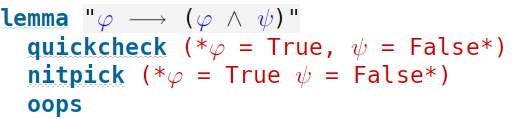
\includegraphics[width=0.5\linewidth]{Isabelle-counter}
    \caption{Example of code in Isabelle testing Nitpick and Quickcheck.}
    \label{img:isabelle-counter}
\end{figure}

\subsection{Lean}
\label{chap:lean}
Lean is a functional programming language that can be used as an interactive theorem prover~\cite{programming}. The structure of the proofs in this tool is very similar to the one presented in~\autoref{chap:prop-deduction}, where it is possible to use rules defined in \gls{ND}, in contrast to Isabelle/HOL. \autoref{img:lean_example} shows an example of a proof in \gls{ND} using Lean's style, while \autoref{tab:lean_example} presents its representation in tree form.

\begin{figure}[htbp]
    \centering
    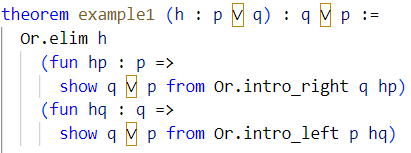
\includegraphics[width=0.5\linewidth]{Lean_example}
    \caption{Example of code in Lean proving \(\{p \lor q\} \models q \lor p \).}
    \label{img:lean_example}
\end{figure}

\begin{figure}[h!]
    \centering
        \[
            \frac{ {\displaystyle {p \lor q}^1 
            \quad \quad \displaystyle \frac{\displaystyle p^2}{q \lor p \strut} (\lor I_l) \strut}
            \quad \quad \displaystyle \frac{\displaystyle q^3}{q \lor p \strut} (\lor I_r) \strut}
            {\displaystyle q \lor p \strut} \quad (\vee E, 2, 3)
          \]
          \caption{Example of a deduction tree proving \(\{p \lor q\} \models q \lor p \).}
          \label{tab:lean_example}
      \end{figure}

Lean also has a tool to automate proofs called Aesop~\cite{leanprovercommunity_2021_github}. Unlike Isabelle/HOL, Aesop can provide a step-by-step proof, but not in the format presented above. The generated proof uses different tactics that are generally not easy to directly map to \gls{ND} rules. However, Aesop allows users to define their own rules/tactics to help with automation. It is possible to restrict the domain of the rules used in the automation process. Perhaps by defining the set of all \gls{ND} rules, we could achieve the desired output, enabling the generation of proofs using only valid rules. Another interesting feature of Aesop is that it allows the user to use part of their proof to generate the rest of it when possible.




